\documentclass[10pt]{article}
\usepackage{cite}
\usepackage[utf8]{inputenc}
\usepackage{url}
\usepackage{hyperref}
\usepackage{amsmath}
\usepackage{amsfonts}
\usepackage{amssymb}
\usepackage{graphicx}
\usepackage{float}
\usepackage{lipsum}
\usepackage{multicol}
\usepackage{xcolor}
\usepackage[font=small]{caption}
\addtolength{\abovecaptionskip}{-3mm}
\addtolength{\textfloatsep}{-5mm}
\setlength\columnsep{20pt}
\graphicspath{ {images/} }

\usepackage[a4paper,left=1.50cm, right=1.50cm, top=1.50cm, bottom=1.50cm]{geometry}

\author{Josh Bailey <josh@vandervecken.com>}

\title{Sequencing the Chiptune Genome}

\begin{document}

        \begin{center}
          {\Large \textbf{Sequencing the Chiptune Genome}}\\
                \vspace{1em}
                Proposal for Thesis\\
                \vspace{1em}
                \textit{
                Ph.D. Student (Music) - Josh Bailey,
                Student Number: 300665818\\
                  New Zealand School of Music—Te Kōkī,
                  Victoria University of Wellington}\\
                \vspace{1em}
                Supervisors\\
                \vspace{1em}
                \textit{
                  Jim Murphy, Victoria University of Wellington\\
                  Dugal McKinnon, Victoria University of Wellington\\
                  Tom White, Victoria University of Wellington}\\
        \end{center}

        \begin{center}
                \rule{150mm}{0.2mm}
        \end{center}

       \begin{abstract}
The Chiptune musical genre (encompassing the sonic aesthetic of early synthesizers and personal computers) is closely connected with the Demoscene, which is an international cultural movement that prizes the competitive and creative realization of new capabilities (in the form of audiovisual performances) using constrained obsolete computers such as the Commodore 64. The Demoscene continues to the present day with regular Demoparties (live events) where innovators demonstrate their discoveries and are recognized for their artistic and technical skill.

Because these obsolete machines are so constrained, very detailed technical knowledge of them is required to identify and exploit capabilities not anticipated by their designers. These capabilities might include the production of complex new audio waveforms from sound hardware not designed to produce them, or fast digital video animation on systems with very small amounts of memory (64KB or less) compared with today’s systems. Performances are often realized as complete machine code programs built byte by byte, by hand, making use of every last CPU cycle available.

The Demoscene therefore has its own history of innovation and culture of competitively producing and building upon past innovations. Demoscene culture continues to be studied ethnographically, and shares with the computer security industry an approach to exploration and exploitation of unintended or undocumented aspects of computer architectures.

This research builds on these cultural themes and prior studies with a computational musicological analysis of a subset of musical performances (as Commodore 64 machine code programs, from Internet accessible community databases), identifying and cataloging the many technical innovations (in the form of machine code that produces unique timbres). The research aims to attribute innovations to authors and groups where possible, tracing the origination, sharing and evolution of techniques over time, with the metaphor of code and its reuse as DNA. While it is proposed not to use machine learning to achieve this, it may be possible to apply techniques including Sparse Autoencoders subject to compliance and regulatory constraints (see below).

Once complete, this analysis will provide the community with an attributed catalog of expressive techniques backed by an reproducible, transparent algorithmic approach (important to the community as a fundamental operating principle of the community is fair, peer recognition of innovation).

The research also aims to produce tools that support further exploration of the Commodore 64 platform, and new performances building on techniques discovered (including interfacing original SID hardware with modern Digital Audio Workstation software without sacrificing the expressibility gained with direct register manipulation).
         \end{abstract}

        \begin{center}
                \rule{150mm}{0.2mm}
        \end{center}

        \vspace{5mm}

\begin{multicols*}{2}

  \section{Introduction}

At first glance, musicological analysis of music on the reputedly best selling computer of all time, the Commodore 64\cite{ieeec64} might appear trivial as the hardware is simple, well documented, and was designed in the late 1970s. Despite this simplicity, the Commodore 64 computer contained an advanced (for the time) synthesizer called the Sound Interface Device\cite{sidpatent} or SID chip. This chip has features recognizable in commodity synthesizers today - multiple voices and waveforms, and software controllable filters. The chip was also integrated into Elektron’s first commercial product, the SIDStation\cite{sidstation}. The SIDStation made SID programming much more accessible to musicians allowing patches to be programmed and sequenced via MIDI, which would otherwise involve writing 6502 machine code. Thanks to continuing innovation in the form of the SIDStation and other tools, interest and creative use of the SID continues to this day beyond its original platform within the Commodore 64.

SID chip programming on the original Commodore 64 involves carefully constructed sequences of changes to memory registers at carefully chosen intervals. These sequences are analogous to DNA - a given performance will include sequences programmed by a composer, either of their own invention (including re-sequencing from another performance that might use similar patches), or sequences recovered from the work of others.

These “DNA” sequences can then be indexed across documented performances, allowing for variation (both variations that produce the same audio output, and variations that produce slightly or vastly different output depending on the precise order in which they are executed). As with DNA, these sequences can be recombined and edited to produce new sequences, compared with other sequences. The effect of changes to a sequence can be determined by executing it on a real or emulated SID and comparing the resulting audio.

The research aims to make a systematic study of all known SID programming sequences (as represented in the High Voltage SID Collection\cite{hvsc} further introduced in Background, High Voltage SID Collection), which will include methods for identifying the same or similar programming techniques across all performances. Since the HVSC collection includes composer names and dates for most performances, it will be possible to realize an evolutionary timeline of techniques (so far as the community provided metadata allow).

One of the conventional approaches to the musicological study of a given genre or set of composers of music, is score analysis. This is a set of techniques for studying written forms of music, representing instructions for musicians to reproduce and interpret a composer’s intentions (for example what range of notes to use and with what cadence). Music21\cite{music21} is a set of tools that enable such high level score analysis and comparison of composition features such as key transitions and beat signatures. The proposed research will go beyond these features and produce new tools that operate at a patch/waveform/microsecond level rather than a MIDI note/bar/measure level.

This level of detail is necessary because the MIDI standard does not define patch parameters such as waveform or FM algorithm, and MIDI-based tools such as Music21, ChiptuneSAK\cite{ChiptuneSAK} or Magenta\cite{Magenta} cannot achieve the level of detail required to capture audio sample level expression. The musicological line between a conventional score (instructions for a musician) versus computer software (very precise instructions to a computer as musician to produce sound) is blurred, but the scope of study is expanded to include very fine details (analogous to the precise handling of the strings of a violin a musician might add as personal expression, beyond what might be written on the score before them).

  \section{Background}

  \subsection{Overview}

It is necessary to describe in greater detail the main research themes in the introduction - the Demoscene community and its values, the Commodore 64 as an instrument and its surprising complexity, and the proposed approach to studying the practice of musical performance and composition within the Demoscene community and on the Commodore 64 specifically. The Demoscene itself as a social phenomenon continues to be studied, as does the Commodore 64 itself.

This research focuses on the technological boundary between these two fields, in not only how the community has expressed its creativity using Commodore 64 as an instrument, but also how that creativity has assumed new forms (and new complexity) over time. Since the Commodore 64 is a computer, this research also studies in effect the creation and innovation of computer programming techniques towards a specific application (creative musical works), using specific sound producing hardware within the Commodore 64 computer (the SID chip).

It is lso necessary to contrast the Commodore 64 with other platforms of the period by describing its relative strength in expressive features and its potential for future exploration and to discuss the degree of intersection between the field of machine learning and this research.

Following this background, the Methodology section will describe precisely how Commodore 64 musicians realize their creativity on the platform, and techniques for quantifying that expression of creativity and how it has evolved and transferred. The Preliminary Work section includes a precise example of how creativity can be described, visualized and demonstrated to rapidly increase over time using those research techniques, and suggests a direction and final form for research findings and potential accompanying creative works.

\subsection{Demoscene Ethnography}

The Demoscene is an ongoing subject of ethnographic research, including the intersection with communities including computer graphics\cite{siggraphdemo} and information security\cite{layerone}. The Demoscene has accompanied and informed the emergence of critical, networked culture with its beginnings in early pre-Internet personal computing\cite{pioneers}, with expansive attitudes towards exploration and information sharing and challenging conventional copyright restrictions.

The Demoscene is also characterized in part by cultural gatekeepers with implicit rules for entry\cite{gatekeepers}, either individually or through Demoparties, which are live competitive events often with specific technical goals. An example of a winning entry is A Mind Is Born\cite{amib}, which realizes a 4 minute audiovisual performance in 256 bytes of code.

\subsection{High Voltage SID Collection}

One way the Demoscene expresses and curates its creative works is through community collections such as the High Voltage SID Collection\cite{hvsc}. This collection represents the perfect subject of creative study because it includes not only the complete creative works themselves but the metadata attributing composer and release date, all in a machine readable format. At the time of writing the collection (version 81) includes over 58,000 songs. The collection also contains some performances which have not yet been attributed to a composer (an explicit research goal is to attribute these performances).

While it cannot be proven to include every known Commodore 64 performance as it relies upon community contributions, informal consultation with Demoscene artists suggest that it is a representative collection, and if there are other sources available they will be accommodated during the research (given that the performances in other collections would also be machine code, they are amenable to the same analysis and tools).

\subsection{Contemporaneous computing platforms}

The Commodore 64 is not the only platform of the period, but is chosen because it is unique in its expressibility for the time and having significant capabilities built in without the user having to add additional hardware.

For example, a competing platform of the period was the ZX Spectrum\cite{attrclash}. This system had only a built in “beeper” speaker with no filters or additional waveforms (though additional hardware was available adding, among other features, FM synthesis). The NES platform, like the SID chip, had multiple waveforms and voices, but no filters, though has been the subject of some musicological research\cite{nesmusic}. For these reasons expressive complexity on these other platforms is limited and so they are not part of proposed research.

\subsection{Machine code and original hardware}

Given the lack of built in sound software in the Commodore 64, the SID chip can only be fully utilized with 6502 machine code\cite{c64digi}, and the chip exhibits significant performance differences (see following) even within units of the same model number and revision.

While several software and hardware emulations of the SID chip exist, the behavior of the original hardware has proven difficult to reproduce exactly and emulator defects continue to be discovered particularly in advanced configurations such as combined waveforms\cite{fixcombwaveforms}. Therefore analysis must include not only methods to work with original hardware, but original machine code as well.

\subsection{Generative synthesis}

Recent work in generative synthesis\cite{neurorack} involves machine learning prediction of audio samples and demonstrates the creative use of patch parameter prediction. A potential research outcome therefore may be a SID generative synthesizer tool that permutes initial SID register state in a creative direction guided by a composer (for example, altering a snare drum patch over time).

\subsection{Machine learning}

The field of machine learning has made rapid advances in the past few years, especially in generative systems. There is every reason to expect continued rapid advances, increased accessibility to artists and the general public, new cultural concerns, and regulatory oversight.

There was informal consultation with artists, machine learning content engineers, and the Centre of Data Science and Artificial Intelligence Te Whiri Kawe in the preparation of this proposal.

Artists expressed both concerns about the potential for capture and decontextualized exploitation of their work without their consent (Morreale et al., 2023), but also an openness to the possibility of new creative tools enabled by the technology\cite{creativityai}. The Centre discussed recent evolving regulation in the European Union making developers of certain models responsible for authenticating model-generated content\cite{euairegs}, and challenges around the policing of the use of open source models. Machine learning engineers (providing tools that can manipulate and generate new content) highlighted the significant responsibilities the proposed regulation has on their industry\cite{nistai}.

The practicality of an open source generative model and its use in the detection of model produced music was also explored (see below). This preliminary work developed these concerns further, in demonstrating the feasibility of generating music and detecting the presence of a given artist in the training data set. These two capabilities are closely coupled at a software/model infrastructure level, without an obvious means of separation being dependent on the same underlying pyTorch code.

These capabilities represent research challenges, partly in accommodating rapid advances (which can be managed by relying on standard industry frameworks), but potentially most importantly by evolving regulation. It can be foreseen that a research or non-commercial open source generative model could be exploited in ways not practical to constrain. This would make it potentially subject not just to philosophical concerns but regulatory ones.

While machine learning research tools have fewer regulatory restraints and may be considered low or limited risk in some creative contexts, given the rapid development of the machine learning field in general (particularly powerful and accessible machine learning frameworks such as pyTorch and TensorFlow), it will become more challenging to delineate research from non-research machine learning tools due to significant shared technical infrastructure. There is also historical precedent of regulation of the export of encryption and other signal processing techniques such as passive radar\cite{munitions}, where research exemptions may not be permitted.

Therefore, while the proposed research will be informed by the field of machine learning, it will in no way rely upon it for the core musicological goals to manage the dual risks of misuse of the research tools and regulatory constraints on research publication. A non-machine learning, conventionally algorithmic tool set will be used as described in Methodology.

However, with the explicit permission from and collaboration with an artist, it may be possible to realize some creative, generative model based work. Ethical, compliance and regulatory concerns will be monitored throughout, and machine learning techniques may be engaged where creatively appropriate (potentially by producing non-open source creative tools not part of the core research activity).

  \section{Methodology}

    \subsection{Overview}

To perform systematic analysis of all SID programming techniques in the HVSC it must be possible to model and describe these techniques and build a kind of DNA database, working from the definition of chiptune DNA established in the Introduction. Tools will be built to gather the DNA along with metadata from where and when it originated, and then enable comparison and sequencing (in the sense of determining the effect of a given DNA sequence).

As raw DNA, the HVSC includes metadata with each performance, including composer names and release dates (where known), and some advisory metadata for a SID player program about how to play the performance, packaged together as a SID file\cite{sidfile}. These metadata include what model of SID chip(s) to use, whether to use timer based playback (see below) etc. A SID file therefore is a complete machine language program that produces sound when played.

In summary the overall methodology will be to understand the structure of all SID files in the HVSC, create tools that parse the files and understand their differences, including understanding the effect of specific sequences of machine language instructions on audio output. 

Once the differences are understood, another tool set will be used to generate visualizations that show evolution of techniques over time and the transfer or coincidental invention techniques among composers. While there are existing tools\cite{ChiptuneSAK} to parse the files, they do not perform such analysis. Informal collaboration with Demoscene artists will be maintained throughout to ensure the research is calibrated against the community’s understanding of techniques and subject to their critical review. These undertakings will make up the bulk of the proposed thesis structure, enumerated below in Chapter 5: Thesis Structure.

Throughout Methodology the term “playroutine” will be used to describe sound producing machine language programs (versus SID files which are containers for playroutines), with the central technique of “register logging” (reading sequences from what the playroutine does to program the SID chip to produce sound). An individual stand alone, comparable, sound producing sequence will be called a “SID Sound Fragment”.

The remainder of this chapter consists of the technical foundations that will support the research including some characterization of the hardware and software used. The Commodore 64 platform’s synthesizer features (in particular the SID chip) will be described including a programming approach. This approach covers how music is performed on the Commodore 64 (playroutines), how composers command the hardware, and how these commands are expressed and also captured for analysis (register logging). A framework for complexity description, comparison and analysis is introduced (the SID Sound Fragment).

\subsection{Playroutines}

A machine language program, or performance, that programs the SID chip to produce sound has been described as a playroutine. The playroutine may be the only program running (such as in a SID file) or it may be cooperatively integrated within another program (for example, a game). Since a playroutine is in the form of a Turing complete computer program it can conceivably take any arbitrarily complex form. However, a common form represented in the HVSC is interrupt driven (a programmable timer triggers an interrupt at some regular interval, which in turn triggers the playroutine to write changes to the SID chip).

\subsection{Register logging}

The most fundamental data upon which the analysis will be based are changes in state (register modifications) of the SID chip. The approach will be to use decompilation tools that intercept all calls between a playroutine and an emulated SID chip. A performance can therefore be represented as a time ordered list of calls, where each call is defined as a 4-tuple. The following table consists of 4 calls.

    \begin{tabular}{|c|c|c|c|}
        \hline
        \rule[-1ex]{0pt}{2.5ex} Time Diff & Chip No & SID Register & Value \\
        \rule[-1ex]{0pt}{2.5ex} (cycles) & & (0-28) & (0-255) \\
        \hline
        \rule[-1ex]{0pt}{2.5ex} 0 & 0 & 24 & 15 \\
        \hline
        \rule[-1ex]{0pt}{2.5ex} 16 & 0 & 0 & 8 \\
        \hline
        \rule[-1ex]{0pt}{2.5ex} 8 & 0 & 1 & 1 \\
        \hline
        \rule[-1ex]{0pt}{2.5ex} ... & ... & ... & ... \\
        \hline
    \end{tabular}

The sequence and content of the calls contain the “patch” information (how a voice is being manipulated - for example switching from a pulse waveform to a noise waveform within 20ms, to produce a percussive sound, as well as score information over a longer time scale (for repeated subsequences producing percussive sounds at regular intervals).
    
\subsection{Voice 3 feedback}

The register log depends upon the SID chip being programmed as a write-only device, where the order of changes is significant, but the performance is not directly aware of the SID chip’s audio output in real time.

However, unlike the other voices, voice 3’s accumulator state can be read from a dedicated 16 bit register. This allows a playroutine to use this state as part of further signal processing or synthesis techniques. For example, this state could be entered into a delay line or queue, and translated into a 4 bit digital sample to be played back via the volume register as delay effect.

It will therefore be necessary to include voice 3’s accumulator state in the register log (see above), along with an additional field indicating if and where the machine code has inspected this state, to enable further analysis of this technique.

\subsection{VICE emulator logging modifications}

The VICE emulator provides a debugging “dump” function that produces logs in the above format, except for the chip number (VICE is modified to add this). The output is post processed to remove redundant state (see below). It will also be necessary to add voice 3 state as above.

\subsection{Sequence segmentation}

The fundamental analysis technique for the thesis is the segmentation of sub sequences of SID register calls at enumerated intervals within the sequence accomplishing an entire performance. Then, identifying repeated sequences and variations and comparing sequences across many thousands of performances.

There are several anticipated stages in segmentation. It is assumed that for a given SID chip (emulated or otherwise) initialized to the same state, that the same sequence of instructions will result in the same output. This assumption will need to be verified throughout as if not correct would invalidate comparison. It is also expected that a set of different sequences may result in the same audio output, so there may be a many to one relationship for a given audio output.

\subsection{Redundant state}

It follows also that there may be sequences that produce no change in audio output (for example, repeatedly writing the same value to a frequency register, or writing a value to a register with less than 8 significant bits). These sequences can be eliminated because by definition their significance is inaudible.

Depending on the machine code making the SID register calls, there may be variation in the time taken between individual items in a sequence (for example, one playroutine might take longer to calculate a new frequency value than another using a different algorithm, even though both playroutines end up calculating the same value). This difference may or may not be audible. A threshold will have to be defined (for example, if SID register changes are accomplished within one audio sample time at 44.1kHz no difference would be observed). Nonetheless, verification of the significance (or non significance) of small differences in timing between the same register calls will be required.

\subsection{Voice multiplexing}

The SID chip has 3 voices, which can be configured in pairs for some FM effects. A given voice may only be paired with a fixed choice of one other (for example, voices 1 and 3 are paired). Due to the very small number of voices available, composers made extensive use of multiplexing, for example executing a percussion sound sequence on voice 1, then executing a simple pulse wave on voice 1 while executing the same percussion sound sequence on voice 2. It is assumed that all single voices are interchangeable, and that all voice pairs are interchangeable, assumptions that must be verified.

Aside from the voices, the SID chip has programmable filters and a 4 bit volume register. All voices are affected by the volume register and can be selectively routed to the filters. There is therefore another kind of sequence state to be considered: individual voice states paired with a specific filter and volume state. These combinations must be modeled for comparison.

\subsection{ADSR envelope bugs}

One of the SID chip’s most documented flaws is a non deterministic ADSR envelope. How the envelope operates upon triggering depends upon its state (which phase it was in with what configuration) when it was last triggered, unless enough time has passed to cause the envelope’s accumulator state to return to its initialized state.

This requires careful management by the composer of ADSR and voice state to ensure the envelope operates, otherwise some envelope phases may be skipped or truncated causing undesired artifacts. As these management techniques are expressed in precisely timed register changes they are captured in the register logging model.

Composer management of this significant hardware flaw is a specific but not exclusive example of a kind of expression to be studied throughout the research.

\subsection{SID Sound Fragment}

Given the SID has an envelope per voice, a convenient way to model a patch is from the envelope being triggered (when the GATE bit is set to 1). This distinguishes a new window (potentially encompassing many other SID writes, for example changing frequencies or waveforms) from a preceding window. This window can be described as a SID Sound Fragment. A SSF must include all information that could influence the output of a voice (including its FM paired voice, and filters).

\subsection{High/low data rate}

Based on preliminary work on complexity assessment (see below) a wide range of complexity in playroutines is anticipated, from very simple, monophonic and mono timbral to extremely complex performances incorporating voice 3 feedback, digital samples and FM synthesis. It is also anticipated that playroutines maybe separated broadly into two groups - low data rate (where the SID chip is programmed strictly on timer intervals of several or perhaps even 10s of milliseconds), and high data rate (where SID chip writes are required potentially several times per millisecond).

The high data rate case is expected to be indicative of very specific synthesis techniques (such as high resolution samples). The low data rate case is expected to be much more common based on preliminary work analyzing HVSC’s metadata.

\subsection{Evolution of SID sample playback}

While the SID chip was not originally specified to include digital sample playback, multiple playback methods have been independently discovered. The most simple method is using the volume register as a 4 bit DAC, while the more complex methods involve using multiple voices together to produce higher resolution waveforms (sometimes in combination with the volume register). In the final thesis document, a section with a a detailed analysis of the techniques and the ancillary techniques (eg. digital signal processing) will be included.

\subsection{SID patch model}

A common patch description will be required to describe all possible SID programming methods, whether low or high data rate. This is likely to be an augmented SSF (SID Sound Fragment, see above), represented at various levels of optional precision and resolution (for example option- ally dropping frequency changes, to compare SSFs with the same waveform combinations regardless of pitch).

Tools will be required to translate SSFs into these various forms, including to external synthesis software (so that extracted patches can be verified or re-used in existing C64 synthesis software).

\subsection{SID patch difference metrics}

With a generic patch model it will be possible to make comparisons in various dimensions, covering cases such as different techniques that achieve similar audio output (perhaps indicative of independent reinvention). As it is possible to generate audio samples from an SSF, it is also possible to “reverse search” from provided audio samples back to SSFs.

\subsection{Visualizing complex and patch dissemination}

With a patch model and varying difference metrics it will be possible to produce graphical representations. For example, a timeline expressing complexity and introduction of techniques, or a directed graph differentiating more common SSF sub-sequences versus less common.

\subsection{Patch programming classification}

The preceding analysis and visualizations will then support a systematic description of each of the distinct programming techniques identified and an elucidation of their propagation over time. Aside from digital synthesis playback such major techniques are anticipated to include ADSR envelope management and single voice combined waveforms.

\subsection{Creative work}

Aside from tools intended for analysis, tools will be developed to creatively permute and rearrange patches/SID Sound Fragments that support the creation of new works in collaboration with Demoscene artists. Anticipated functionality of such tools would include the evolution over time of the timbre of a sound, such as a drone texture, or the efficient exploration of complex timbres by automatically identifying new, unique sequences not found in existing works, which would be another dimension of contribution to the Demoscene community.

\subsection{Methodology summary}

In the development of this proposal some rudimentary tools have been developed (see following section), which have in turn also suggested probable analysis components such as the SID Sound Fragment as part of the DNA sequencing metaphor. The proposed SID Sound Fragment could be compared between performances and composers at varying levels of precision. The proposed Methodology has been developed around the High Voltage SID Collection, but can be applied to any Commodore 64 software, so the research could be expanded to other collections.

\section{Preliminary work}

\subsection{Overview}

The tools and concepts discussed in Methodology were developed and applied to the High Voltage SID collection as discussed below. The goal of the preliminary work was to informally gauge artistic interest and value of the research and obtain a high level understanding of complexity of performances (specifically, whether the level of complexity was sufficient to research).

\subsection{Decompilation}

Basic tools have been assembled (see above) based on the VICE emulator\cite{asidvice} to provide scope for the research, and to inform the initial SSF/sequencing concept.

\subsection{sidtableflip}

An experimental model named sidtableflip\cite{sidtableflip}, based on the pyTorch framework, has been developed. This model is capable of probabilistic prediction of music based on register logs, in snippets of 30 to 60s. This model exercises the register logging methodology, verifies research platform hardware and software requirements (including a dedicated RTX 4090 GPU), and provides a testing method for future composer and technique identification techniques as well as potential generative creative works.

sidtableflip is based on pyTorch reference text generator’s Transformer architecture (Zhang, 2019), with the most significant difference in tokenizing the register log - each unique register assignment in the log is a token. A convention in text generation models is incorporation of punctuation with each word (e.g. assuring ”word,” and word!” are different tokens with their accompanying context.)

Since sidtableflip incorporates the time since the last register change with each token,  it effectively includes the musical ”punctuation” in the form of cadence and tempo. A 4 layer Transformer with 2 attention heads and 256 embedding dimensions, predicting 2048 call sequences, takes approximately 1 day to train over 64 songs, comprising a sequence 3 million tokens long with approximately 20000 unique tokens.

\subsection{Waveform complexity visualization}

A preliminary analysis has been performed year by year, to show the overall increase in expression and complexity in performances over time by producing a directed graph summarizing all the state transitions of each SID voice control register (the register which configures a voice to use certain waveforms or be modulated by another voice, and whether to restart the ADSR envelope).

In the very early years, state transition complexity is quite low and easy to visualize as the number of performances produced is small and composers have not yet explored all possibilities. Complexity very rapidly increases over the next few years. The following diagrams represent all performances produced in the years 1982, 1983, and 1984, and while not the final research product are illustrative (the size of the connection between states is proportional to how often that state transition is used).

The research will explore this more deeply with tools that can selectively focus on different types and sources of complexity (for example, show how a given composer’s technique has evolved over time, and/or how the set or related techniques have evolved, such as combining selected waveforms). This may support a kind of visual complexity notation.

\begin{figure}[H]
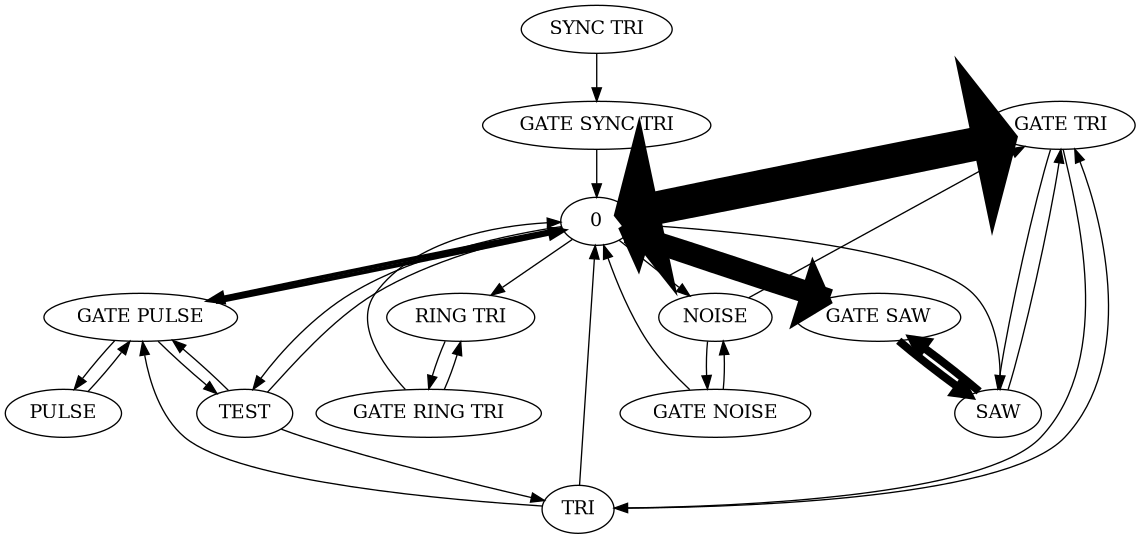
\includegraphics[width=0.5\textwidth]{1982}
\caption{1982}
\end{figure}

\begin{figure}[H]
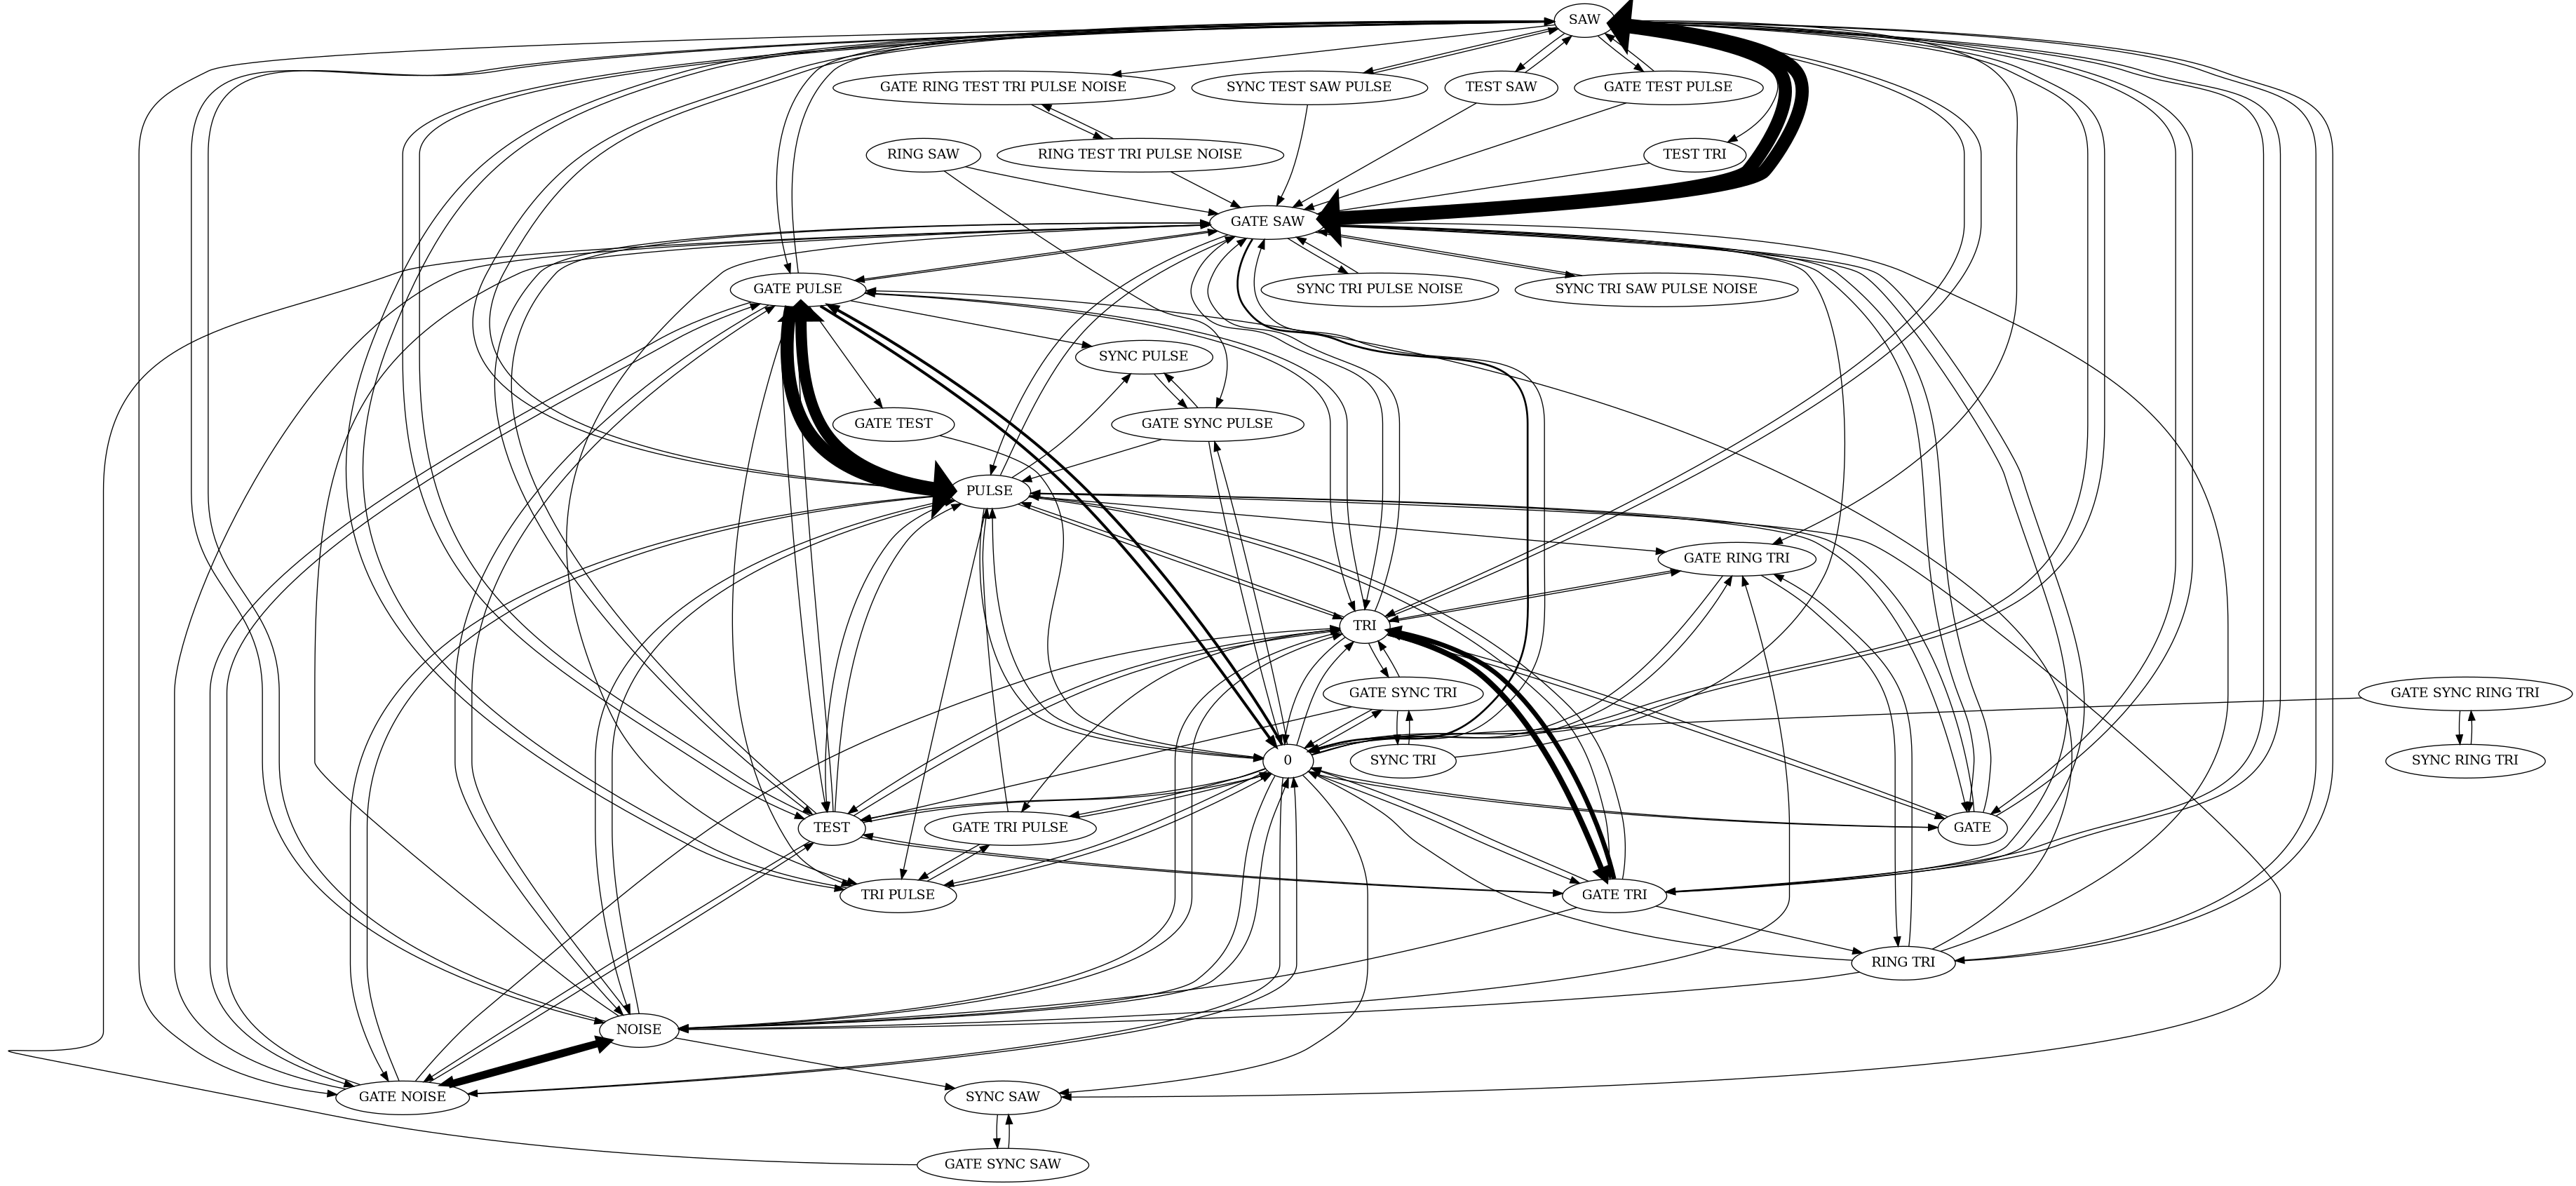
\includegraphics[width=0.5\textwidth]{1983}
\caption{1983}
\end{figure}

\begin{figure}[H]
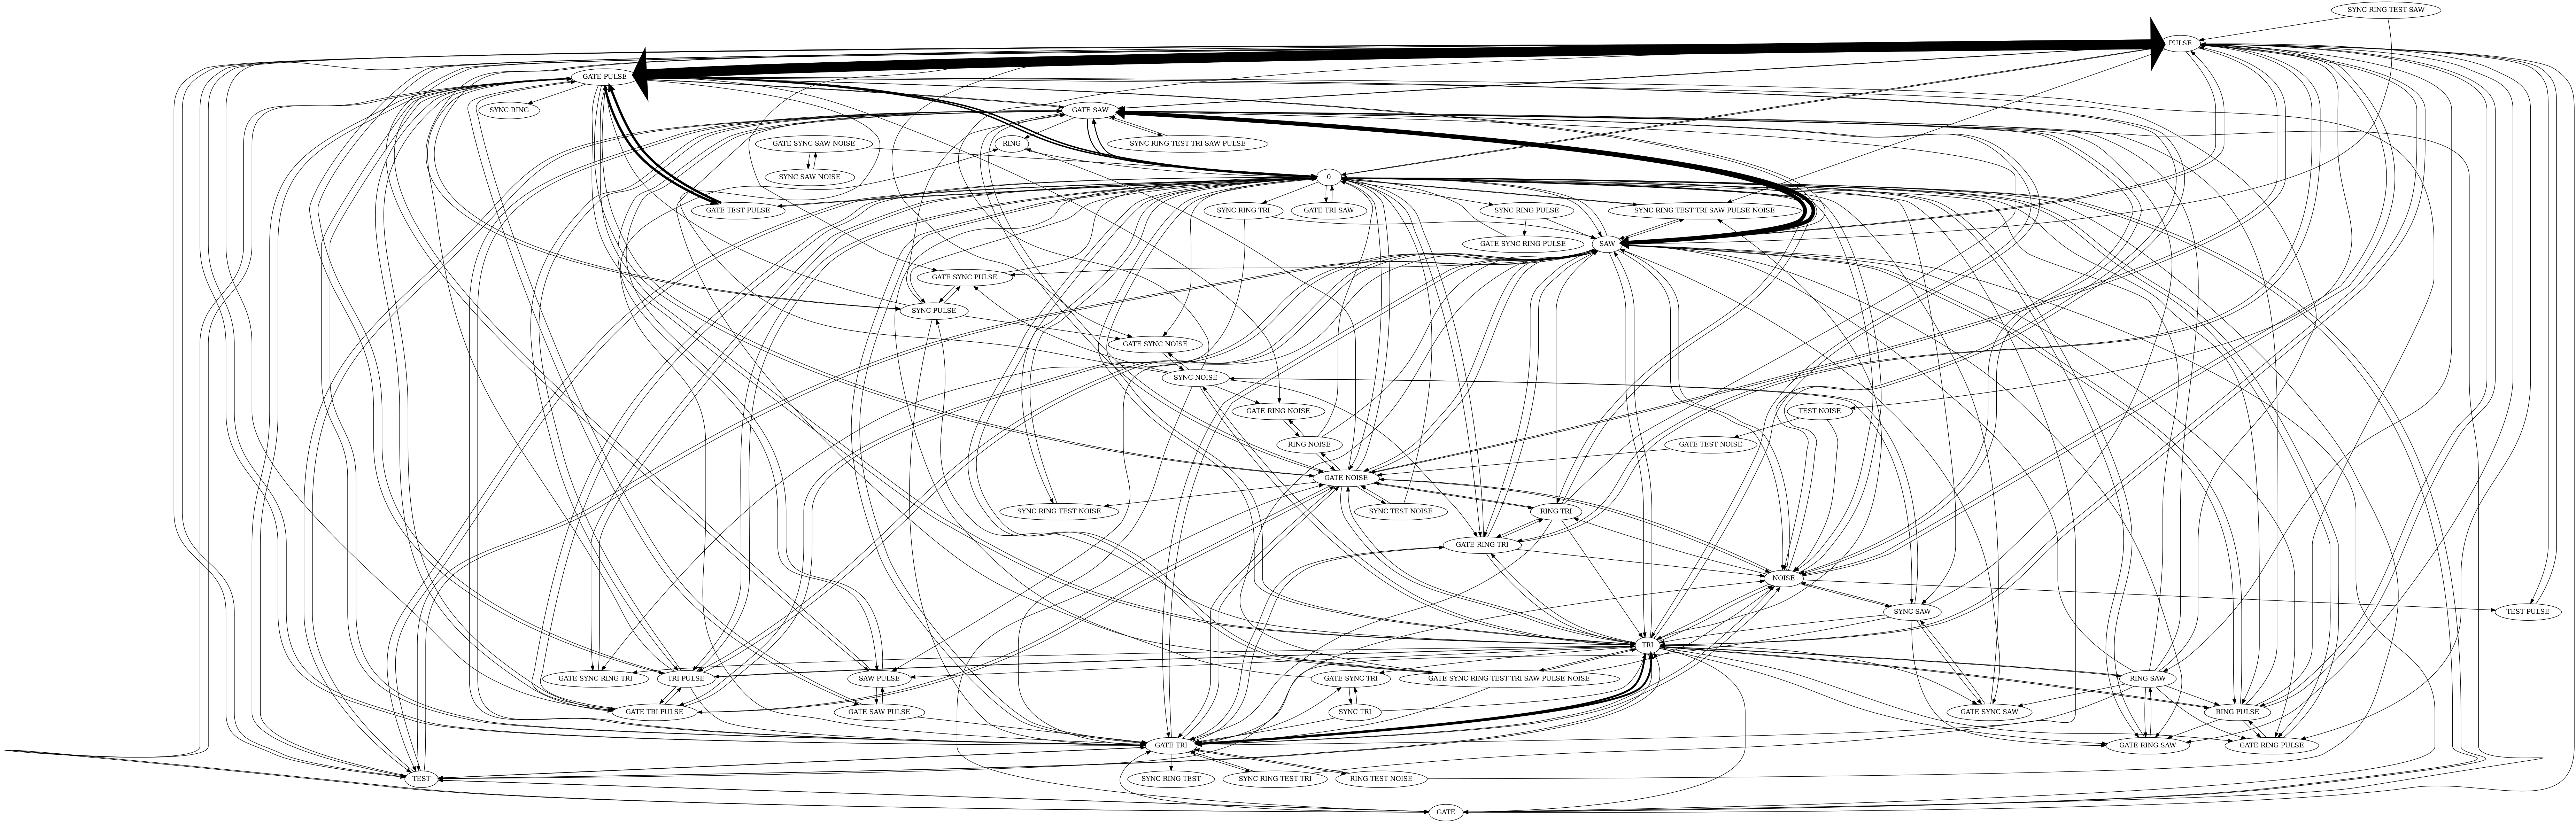
\includegraphics[width=0.5\textwidth]{1984}
\caption{1984}
\end{figure}

\subsection{Preliminary work summary}

In development of the proposal the complexity and scope of the dataset was explored, prototype tools were developed, and there was extensive engagement with influential artists in the field. Two important results were obtained, firstly that artists saw the value of algorithm-assisted attribution to their community, and also the value of future tools that could assist in the discovery of new expressive techniques. Secondly, the prototype research tools support the assertion that a complete examination and analysis of the entire dataset is practical to achieve, and that despite the simplicity of the underlying technology, that there is complexity of research interest.

\section{Thesis structure}

The thesis will be arranged as follows, with an approximate time budget relative to a 3 year timeframe. The bulk of the time is anticipated to be spent on the identification of techniques themselves followed by the study of how the techniques have evolved and propagated between artists.

  \begin{tabular}{|l|l|l|}
        \hline
        Section & Description & Time budget \\
        \hline
        Introduction &  & 5\% \\
        \hline
        Demoscene culture & The Demoscene and its connection to innovation. & 5\% \\
        \hline
        SID programming & SID hardware and its programming paradigm. & 5\% \\
        \hline
        Methodology & Development of tools and process for SID musicology. & 20\% \\
        \hline
        Composer techniques & Unique techniques and timbres identified. & 25\% \\
        \hline
        Composer identification & Attribution of techniques and their propagation. & 25\% \\
        \hline
        Creative applications & Production of a generative work in collaboration with a Demoscene artist.  & 10\% \\
        \hline
        Conclusion and future work & Summary of the research and potential for further research. & 2.5\% \\
        \hline
        Bibliography/references &  & 2.5\% \\
        \hline
  \end{tabular}

  \subsection{Dissemination}

  The analysis suite of tools used in the research will be open sourced, and may take different forms depending on reception by the Demoscene community. For example some of the register logging functionality may be integrated with the main line version of VICE emulator, while other tools will be maintained separately. This open sourcing will facilitate collaboration with Demoscene artists and support criticism and improvement of the attribution techniques.

  An explicit goal is a collaboration with an artist which may take the form of a partially generative performance, and/or a tool that enables an artist to identify the use of a particular technique in any arbitrary piece of music.

  The research will be proposed for presentation at a Demoparty in 2025, where Demoscene artists will be engaged for their critical feedback.

  \subsection{Datasets}

Aside from performance opportunities that may arise during the course of the research, the primary dataset to be produced (aside from the visualizations described above), together with a tool will enumerate the relationships between a given performance and all other known performances.	The tools and resulting research are proposed to be submitted for publication progressively and iteratively throughout (for example, starting with a paper discussing waveform complexity over time). u

\section{Novel contributions and conclusions}

Existing computational musicological frameworks operate at the level of a conventional score, (without consideration of synthesizer patch configuration), or at the audio feature level (what pitches are most perceptible, how intensity changes over time, etc).

This research introduces a rich new level of musicological detail in analyzing expression in electronic music, down to the precise instructions used by composers to originate each sound. While the central research platform, the Commodore 64, is limited, many of the techniques should apply to more complex systems (for example, analysis of Ableton Live set files).

Since also the central research approach involves attribution of the output of machine code programs, it may have non-musical applications (for example in computer security, attributing authorship of very low level computer malware).

Finally, this research will support the recognition and attribution of innovation within the Demoscene community, suggest new areas of expression to explore, and make it easier with tools for Demoscene musicians to build upon each other’s work while retaining attribution of contributions. With future work, these benefits may be transferable to practices for other kinds of electronic music.


\clearpage


\end{multicols*}

\nocite{*}
\bibliographystyle{plain}
\bibliography{sidbasecode_proposal}


\end{document}

% LocalWords:  PCM timeline HVSC Dessimenation Ableton APA citet nzsm
% LocalWords:  programmatically citep phd ADSR
